\chapter{Anforderungsanalyse}

In der durchführenden Analyse wird ein neues Bestell- und Verwaltungssystem Konzept erläutern. Auf der Basis der IST-Analyse wird eine Verbesserung mit aktuellen Webtechnologie und Verfahren durchgeführt.
In diesem Kapitel wird man sich die entstehenden Probleme und Optimierungspotenzial näher anschauen.

Das neue Bestellsystem soll nicht kompliziert sein, sondern Benutzerfreundlich. Die Optionen sollen klar gezeigt werden und einfach sein. Sicherheit ist einen wichtigen Teil der guten webbasierte Entwicklung, aus diesem Grund werden zusätzliche Prüfungen in dieser Richtung entwickelt.
Die Auftragsverwaltung und Kundenübersicht werden mit denselben Funktionen bleiben.
Das ganze Konzept wird aus einer Umbraco-Instanz heraus verwaltet.
In den folgenden Unterkapitel werden die oben beschriebene Anforderungen erweitert und erläutert.


\section{Paket A}
Aktuelle Software ergibt sich dem Auftraggeber wenige Möglichkeiten Frontend zu ändern. Es wurde immer ein Entwickler benötigt, um etwas geändert zu werden. Ein Beispiel dafür ist, dass der Auftraggeber nicht den Schrift oder die Farbe des Textes editieren konnte.
   
In diesem Unterkapitel wird eine volle Freiheit des Auftraggeber zur Verwendung der Tätigkeiten angefordert. Es wird besonders darauf geachtet, dass die Möglichkeiten zu ändern und editieren, erhalten bleiben. Als Beispiele wurden Schriftart und Farbe vorgegeben.

Es wird die Verwendung vom Grids, Macros und Formulare empfohlen.
Diese und weitere Begriffen werden im nächsten Kapitel erläutert.


\section{Paket B}


\subsection{Kundenverwaltung}

In diesem Unterkapitel wird es mit den Anforderungen beschäftigt, die der Auftraggeber gestellt hat, um die Kundenaktivitäten besser kontrollieren zu können. Eine eigene Seite wird auch erstellt, in der Kunden Bestellungen erstellen und einsehen können oder Nachrichten verschicken oder lesen können.

\subsubsection{Kundenerfassung}
Hier wird es die Anforderungen zu den Onlinebestell-System und Kunden Übersicht beschrieben.
\begin{enumerate}
	\item Der Kunde kann sich bei der Erstbestellung registrieren und bekommt eine PIN zugeschickt. Bei jede weitere Bestellung kann er sich mit seiner E-Mail und der PIN einloggen. Das, was beachtet werden muss ist, dass beim Bestellen die Mail geprüft werden muss und ein Hinweis ausgegeben werden soll, wenn die Mail schon in der Datenbank bereits existiert. Die Neukunden kommen in der Bestellübersicht des Auftraggebers in einer gesonderten Übersicht und sie müssen von ihm bestätigt oder übernommen werden. Danach kann der Kunde sich einloggen.
	In den Abbildungen \ref{fig:registerForm} und \ref{fig:anmeldeformular} sind die Register- und Anmeldeformular zu sehen.
	In den vorgegebenen Anforderungen ist zu diesem Punkt, nichts zu ändern. Die Funktionalitäten und Aktivitäten müssen dieselben bleiben.
	
\end{enumerate} 

\subsubsection{Kundenansicht}

\begin{enumerate}
	\item Wenn der Kunde vom Auftraggeber verifiziert wird, kann sich mit seinen E-Mail und PIN einloggen. Er kann seine aktuelle und vergangenen Bestellungen einsehen. Ein Kontaktfenster wird verwendet, über das die Kommunikation und Absprache läuft. Der Auftraggeber kann entweder allgemeine Information seinem Kunde schreiben oder Kundenspezifisch. Die Abbildung \ref{fig:KundenAnsicht} stellt die bisherigen Kundenansicht dar 
	Das sind die alte Funktionalitäten. Es wird angefordert, sie nicht geändert zu werden, aber die Kunden sollen über Member-Section im Umbraco abgebildet werden.  
\end{enumerate} 

\subsubsection{Auftraggeber-Ansicht}

\begin{enumerate}
\item Der Auftraggeber hat eine Kundenübersicht, die er filtern kann. In der Detailansicht sieht er die Infos zum Kunden wie Bestellverlauf und kann von der Ansicht heraus E-Mails an den Kunden senden (Mail-Vorlage oder frei gestaltbar). Anschaulicher wird im Abbildungen \ref{fig:KundenDatei} und \ref{fig:KundenEditor} dargestellt.
In dem neuen Konzept wird angefordert, die Funktionalitäten von der alten Software gleich zu bleiben.
\end{enumerate} 

\subsubsection{Kommunikation}

\begin{enumerate}
	\item Über die Option „neue Nachrichten“ kann der Auftraggeber mit seinen Kunden kommunizieren und Absprachen zu den Aufträgen treffen.
	\item Für das neuen Konzept soll eine neue Kommunikationsmethode für die alte Funktionalitäten mit Filtern (gelesen, nach Kunden suchen usw.) integriert werden. Der „Chat“ sollte auch aus der Kundenkartei-Ansicht funktionieren und die Kommunikation soll an einen Auftrag gebunden sein. 
	Die Kommunikationsübersicht wird in Abbildung \ref{fig:NachrichtErscheint} illustriert. 
	\begin{figure}[h]
		\centering
		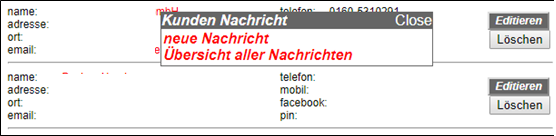
\includegraphics[width=0.7\linewidth]{Graphics/newNach.png}
		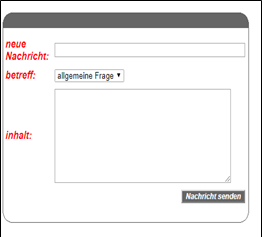
\includegraphics[width=0.7\linewidth]{Graphics/newNachr.png}
		\caption[Neue Nachricht]{Die bisherige Eingabemaske für die Nachricht}
		\label{fig:NachrichtErscheint}
	\end{figure}

\end{enumerate} 


\subsection{Artikelverwaltung}

\subsubsection{Artikel erfassen, ändern und löschen}

\begin{enumerate}
	\item Der Auftraggeber kann in einer recht einfachen Maske Artikel verwalten (online-editor). Es gibt nur zwei Kategorien: Arrangements und Artikel-Standard. Im Moment sind die Arrangements noch nicht mit den Webseiten gekoppelt.
	\item Ein Arrangement besteht aus Kategorien (fest vorgegeben) und Positionen und kann sich darin unterscheiden, ob Kunden Positionen auswählen dürfen oder nicht.
	\item Es wird angefordert, der Artikel einfacher verwaltet werden zu können können und die Artikelseite der Webseite soll direkt mit dem Artikel gekoppelt sein.
	
	Bisherige Übersicht für den Artikel ist in der Abbildungen \ref{fig: Online-EditorUebersicht} und \ref{fig: Editor-Menü2} zu sehen.
	
\end{enumerate} 


\subsection{Auftragsverwaltung}

\subsubsection{Übersicht}

\begin{enumerate}
	\item Der Auftraggeber hat eine Übersicht über seine aktuellen Aufträge. Für jede Art von Auftrag (neu, bearbeitet, alte und fällig) gibt es ein Select-Befehl.
	\item Diese Ansicht soll in einer eigenen Umbraco-subsection umgesetzt werden. Die Artikeldatenbank soll von Access nach SQL transportiert werden. Es muss eine neue Zuordnung Kunde zu Umbraco-Member geben.
	In den Abbildung \ref{label} ist die Übersicht zu sehen.
\end{enumerate} 



\subsubsection{Detailansicht}

\begin{enumerate}
	\item In der Detailansicht kann der Auftraggeber den Auftrag bearbeiten, den Status ändern, Positionen editieren / hinzufügen und löschen, dem Kunden Freigaben erteilen (z.B. Aussuchen der Positionen) und eine Rechnungsnummer vergeben.
	\item Der Auftrag muss auf vier Seiten ausdruckbar (genau vor-gegeben) sein.
	\item Die Begrifflichkeiten von zweitem Blatt müssen für Auftraggeber zu Verfügung gelassen werden, damit er sie selbst ändern kann.
	\item Quick-Icons erleichtern die Kommunikation mit dem Kunden und die Anpassung an dessen Auswahl zu Auftragsbeginn (z.B. Änderung Serviceauswahl).
	\item  Diese Ansicht soll in einer eigenen Umbraco-subsection umgesetzt werden.
	
	Detailansicht wird in der Abbildung \ref{label} dargestellt.
\end{enumerate} 


\subsection{E-Mail-Verwaltung}

\begin{enumerate}
	\item Hier kann der Auftraggeber E-Mail Vorlagen mit Platzhaltern definieren, die er dann in der Kundenkommunikation auswählen kann.
	\item Es gibt ein Form für Terminanfragen über die Webseite. Diese erzeugen eine Mail an den Auftraggeber. Dieser muss in der Mail nur einen Link betätigen, um die Anfrage zu bestätigen. Dies hängt auch mit dem E-Mail Verwaltungssystem zusammen.
	\item Diese Ansicht soll in einer eigenen Umbraco-subsection umgesetzt werden.
	Anschaulicher wird im Abbildung \ref{label} dargestellt.
\end{enumerate} 



\subsection{Umsatzverfassung}
\begin{enumerate}
	\item Hier kann der Auftraggeber sich die Umsätze der letzten Monate / Jahre, die über die Aufträge zustande gekommen sind, an-schauen. Dabei ist es wichtig, dass diese Datensätze nicht direkt an die Aufträge gekoppelt sind, sondern aus einer extra Tabelle kommen, die der Auftraggeber auch selbst noch editieren kann.
	\item Diese Ansicht soll in einer eigenen Umbraco-subsection umgesetzt werden.
	In der Abbildung \ref{label} wird die Umsatzerfassung dargestellt.
\end{enumerate} 


